\chapter{Proposta} \label{cap:proposta}

Como visto no Capítulo 2, a mineração de opinião pode ser usada para explorar o conteúdo digital gerado pela nossa sociedade todos os dias em redes sociais, através de técnicas utilizando Processamento de Linguagem Natural e \textit{Machine Learning}, principalmente. Com este fato surge a oportunidade de explorar novas ferramentas na
solução de problemas que envolvem pesquisas de opinião de forma geral.

Neste trabalho propõem-se um \textit{framework} que torna possível fazer pesquisas de opiniões em língua portuguesa sobre qualquer tema que seja rastreável a partir de uma \textit{hashtag} no Twitter.
Para tal é necessário que o \textit{framework} criado seja capaz de:

\begin{enumerate}
	\item Coletar \textit{tweets} escritos em língua portuguesa que contenham uma determinada \textit{hashtag};
	\item Armazenar as mensagens em uma base de dados;
	\item Classificar as mensagens de acordo com a polaridade: negativo, neutro e positivo;
	\item Extrair \textit{insights} que auxiliem a tomada de decisão a partir da massa de dados classificada.
\end{enumerate}

\section{Coleta de dados}
A plataforma do Twitter conecta aplicações e sites com seus dados através de diversos serviços. Para este trabalho, a principal fonte de dados será sua API REST, que possui uma excelente documentação disponível em \cite{twitterapidocs}. Através dela é possível acessar informações de usuários e \textit{tweets}, assim como escrever novas mensagens. Além disso, a API conta com um mecanismo de busca poderoso, que será fundamental para a coleta de dados. Os dados são entregues no formato \ac{JSON}.

\subsection{Autenticação}

Para que ter acesso à API é necessário possuir uma conta no Twitter e criar uma aplicação - através do próprio site \cite{twitterapp} - que utilizará o protocolo de autenticação OAuth\cite{oauth} para acessar os dados do Twitter se passando pelo usuário em questão. O objetivo do protocolo OAuth é permitir que uma aplicação se autentique em outra "em nome de um usuário". A aplicação pede permissão de acesso ao usuário, que possui a escolha de conceder permissão ou não. Um ponto importante: o usuário não precisa informar a sua senha para se autenticar, portanto a permissão continua vigente caso a senha do usuário se altere, o que permite que a aplicação não precise de manutenção neste caso, tornando-a mais resiliente. A autenticação por meio do OAuth necessita de três passos:

\begin{enumerate}
	\item Aplicação cliente obtém chave de autenticação;
	\item Usuário autoriza aplicação cliente na aplicação servidora;
	\item Aplicação cliente troca a chave de autenticação pela chave de acesso;
\end{enumerate}

Após o processo de criação da aplicação, é criado um \textit{token} de acesso que deve ser utilizado pelo sistema que deseja se autenticar no Twitter em nome de um usuário. Este \textit{token} deve ser incorporado em cada requisição à API do Twitter para autenticar a mesma e dizer ao Twitter qual é a fonte do acesso.

\subsection{Limite de requisições}
A fim de evitar grande concentração de requisições em seus serviços, o Twitter implementa um limitador em sua API \cite{twitterrequestlimit2016}. São permitidas até 180 requisições por janela, que dura 15 minutos. Caso o limite seja ultrapassado, o serviço passa a retornar um erro na resposta, até que a janela de 15 minutos se renove.

A partir da versão 1.1 da API, novos cabeçalhos \ac{HTTP} são retornados provendo \textit{feedback} sobre os limites para requisição. Este recurso permite que o código consiga entender em que momento da janela se encontra, quantos requisições ainda podem ser feitas neste período de tempo e quanto é necessário esperar para poder fazer novas requisições. Os cabeçalhos em questão são:

\begin{itemize}
	\item \textit{X-Rate-Limit-Limit}: A faixa limite para o requisição em questão;
	\item \textit{X-Rate-Limit-Remaining}: O número de requisições que ainda restam para a janela de 15 minutos;
	\item \textit{X-Rate-Limit-Reset}: O tempo restante dentro da janela de requisições atual, dado em segundos.
\end{itemize}

\subsection{Arquitetura}

Neste trabalho, como o objetivo é coletar \textit{tweets} postados sobre uma \textit{hashtag} em tempo real para utilizá-los como matéria-prima para análise de sentimento, é muito importante aproveitar ao máximo cada janela de requisições. Por este motivo, o sistema que coleta os dados da API do Twitter foi inspirado no modelo produtor-consumidor\cite{jeffay1993real} visando minimizar as perdas que podem acontecer em momentos de pico - como o começo ou clímax do evento, onde o volume de mensagens é maior, como veremos a frente no Capítulo 4 - e se necessário, escalar de forma simples durante os mesmos. 

\subsubsection{Produtor-consumidor}

O problema descreve dois processos, o produtor e o consumidor, que compartilham um recurso em comum usado como uma fila - um tipo particular de coleção de dados onde a primeira a entidade a entrar é a primeira a sair ou \ac{FIFO} . A função do produtor é gerar trabalho a ser executado pelo consumidor. O volume de trabalho gerado e executado pelo sistema é controlado pela fila, que armazena as entidades ou "tarefas" a serem executadas. Essa abordagem permite que o sistema escale apenas até a sua capacidade, visto que a fila possui um tamanho fixo que caso seja ultrapassado, pode simplesmente descartar as mensagens adicionadas após este momento. Outra característica importante é a escalabilidade. Conforme os processos produtor e consumidor evoluem, surge a necessidade de aumentar a quantidade de produtores ou consumidores de forma independente.

Neste trabalho, para explorar o potencial máximo da janela de requisições foi criado um processo produtor que envia para a fila mensagens para que consumidor acesse à API do Twitter de forma que sejam feitos sempre as 180 requisições que são permitidas no intervalo de 15 minutos. Assim a responsabilidade de cada processo fica bem definida - o primeiro responde pelo volume de requisições e o segundo por realizar a requisição e entender a resposta. Para definir qual intervalo de tempo deveria ser usado para que o produtor envie mensagens à fila, foi feita uma conta simples:

$$ \frac{180}{15} = 12 \textit{ requests}_{/minuto} $$

Logo, o produtor precisa adicionar uma mensagem na fila a cada 5 segundos, para que o limite de 180 requisições seja respeitado.

\begin{figure}[H]
	\centering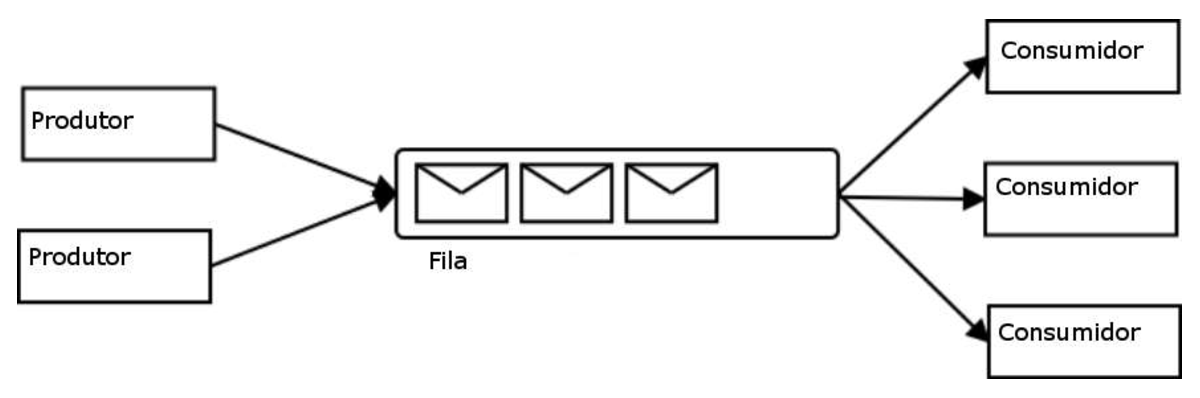
\epsfig{file=figuras/[competing-consumers-eps-converted-to_importada_.eps, width=15cm}
	\caption{Exemplo de arquitetura produtor-consumidor. Fonte: Apache ActiveMQ( http://activemq.apache.org/clustering.html)}
	\label{time}
\end{figure}


\subsection{Busca}
Dentre os principais serviços da API do Twitter está a busca. Com ela, é possível consultar de diversas formas os principais \textit{tweets} ou mais recentes. Dentro de sua documentação, existe um guia completo de como utilizar a API  para extrair os resultados desejados \cite{twittersearchapi} das mais diversas formas. 

\subsubsection{Parâmetros adicionais}

Como abordado acima, a API possui diversos parâmetros que podem ser usados para que o usuário chegue a um conjunto de dados mais próximo da sua necessidade:

\begin{itemize}
	\item \textit{\textbf{result\_type}}: permite escolher se o resultado da busca será representado pelos \textit{tweets} mais populares (\textit{popular}) ou mais recentes (\textit{recent});
	\item \textit{\textbf{geocode}}: permite buscar por uma determinada latitude, longitude e raio, respectivamente, separando-os por vírgula. ex: geocode=-22.912214,-43.230182,1;
	\item \textit{\textbf{lang}}: restringe os \textit{tweets} buscados a um idioma específico. ex: lang=pt;
	\item \textit{\textbf{since\_id }},  \textit{\textbf{max\_id }}, \textit{\textbf{count}} e \textit{\textbf{until}}: possibilita iterar através dos resultados quando existe um grande números de \textit{tweets} a percorrer. De acordo com a concorrência e o volume, esta tarefa pode ficar mais complicada. Uma leitura recomendada sobre o uso destes parâmetros pode ser encontrada em \cite{workingwithtimelimes}.
\end{itemize}

Como o objetivo deste trabalho é coletar novos \textit{tweets} conforme eles vão sendo postados, foi necessário utilizar apenas dois parâmetros da API de busca: \textit{count} e \textit{since id}. O primeiro tem o objetivo de garantir o número máximo de registros retornados pela API e o segundo define de onde se pretende partir para buscar novos \textit{tweets}, evitando que mensagens repetidas sejam coletadas. Um exemplo de requisição pode ser visto abaixo:

\url{https://api.twitter.com/1.1/search/tweets.json?q=#oscars2016&count=100&since_id=123456789}

Neste caso, a API retornará os 100 \textit{tweets} publicados desde o \textit{tweet} com identificador (\textit{id}) "123456789".

\subsubsection{O problema com a detecção automática de idioma do Twitter}

O escopo deste trabalho determina que o objeto de estudo são apenas mensagens escritas em língua portuguesa. Para tal é preciso utilizar o parâmetro \textit{lang}, por exemplo:

\url{https://api.twitter.com/1.1/search/tweets.json?q=#oscars2016&lang=pt&result_type=recent}

Porém, realizando alguns testes na API do Twitter, foi detectado que ao submeter algum \textit{tweet}, alguma rotina dentro do próprio Twitter atribui um idioma à mensagem automaticamente. Nos testes conduzidos durante este trabalho foi identificado que em mensagens curtas - algo recorrente no Twitter - esta atribuição apresenta resultados aquém do esperado na identificação do idioma, visto que as poucas palavras contidas na mensagem podem ser comuns a mais de um idioma. Por conta disso foi decidido que o filtro de idioma não seria utilizado. Esta decisão pode mudar de acordo com o evento monitorado ou com o escopo do estudo.

\subsubsection{Escalando de forma horizontal}

Por uma questão de desenho da API de busca, cada requisição é capaz de trazer no máximo 100 \textit{tweets}, o que nos dá ao total uma carga máxima de até 1200 novos \textit{tweets} por minuto. Para as análises feitas durante este trabalho este número se mostrou mais do que suficiente. Como dito anteriormente, se fosse necessário escalar este sistema para monitorar um evento maior, seria necessário apenas obter um saldo maior de requisições junto a API do Twitter - adicionando mais \textit{tokens} de usuário e criando uma espécie de "rodízio" de autenticações, por exemplo - e escalar o número de consumidores do processo de acordo com a demanda. Uma boa maneira de detectar se isso seria necessário é acompanhar quantos \textit{tweets} novos são coletados a cada requisição. Como utilizamos o \textit{id} do último \textit{tweet} capturado como referência para os novos, se a cada requisição o número de novos \textit{tweets} com grande frequência coincidir com o limite da API, temos um indício de que o volume de novas mensagens no Twitter está excedendo a capacidade do sistema de coletá-las e que o excedente está sendo perdido.

\section{Armazenamento}
\label{proposta:armazenamento}
A resposta da API de Busca é dada no formato JSON e cada objeto - que corresponde a cada \textit{tweet} - segue o seguinte formato e conta com diversas informações sobre o mesmo: 

\begin{lstlisting}[style=json, frame=single]
{
	"_id" : "56d388096861353c1b061fe2",
	"contributors" : null,
	"truncated" : false,
	"text" : "Leonardo DiCaprio com o #oscars eh igual a Katy Perry com o Grammy #OscarsNaTNT",
	"is_quote_status" : false,
	"in_reply_to_status_id" : null,
	"id" : 704091511902834688,
	"favorite_count" : 0,
	"source" : "<a href=\"http://twitter.com/download/android\" rel=\"nofollow\">Twitter for Android</a>",
	"created_at_datetime" : ISODate("2016-02-28T20:51:12.000Z"),
	"retweeted" : false,
	"coordinates" : null,
	"created_at_timestamp" : 1456714272.0000000000000000,
	"entities" : {
		"symbols" : [],
		"user_mentions" : [],
		"hashtags" : [{
			"indices" : [ 24, 31 ],
			"text" : "oscars"
		}, 
		{
			"indices" : [ 66, 78],
			"text" : "OscarsNaTNT"
		}],
		"urls" : []
	},
	"in_reply_to_screen_name" : null,
	"id_str" : "704091511902834688",
	"retweet_count" : 0,
	"in_reply_to_user_id" : null,
	"favorited" : false,
	"user" : {
		"follow_request_sent" : false,
		"has_extended_profile" : true,
		"profile_use_background_image" : false,
		"id" : 2786117482,
		"verified" : false,
		"profile_text_color" : "000000",
		"profile_image_url_https" : "https://pbs.twimg.com/profile_images/700450356141158404/xA-mRqp7_normal.jpg",
		"profile_sidebar_fill_color" : "000000",
		"is_translator" : false,
		"entities" : {
			"description" : {
			"urls" : []
			}
		},
		"followers_count" : 156,
		"protected" : false,
		"location" : "Um lugarzinho no fim do mundo",
		"default_profile_image" : false,
		"id_str" : "2786117482",
		"lang" : "pt",
		"utc_offset" : -28800,
		"statuses_count" : 6171,
		"description" : "Uuuumm ta estilosa!",
		"friends_count" : 192,
		"profile_background_image_url_https" : "https://abs.twimg.com/images/themes/theme1/bg.png",
		"profile_link_color" : "9266CC",
		"profile_image_url" : "http://pbs.twimg.com/profile_images/700450356141158404/xA-mRqp7_normal.jpg",
		"notifications" : false,
		"geo_enabled" : false,
		"profile_background_color" : "000000",
		"profile_banner_url" : "https://pbs.twimg.com/profile_banners/2786117482/1456444936",
		"profile_background_image_url" : "http://abs.twimg.com/images/themes/theme1/bg.png",
		"name" : "Padeira Estilosa",
		"is_translation_enabled" : false,
		"profile_background_tile" : false,
		"favourites_count" : 6095,
		"screen_name" : "naycordeir",
		"url" : null,
		"created_at" : "Fri Sep 26 18:43:47 +0000 2014",
		"contributors_enabled" : false,
		"time_zone" : "Pacific Time (US & Canada)",
		"profile_sidebar_border_color" : "000000",
		"default_profile" : false,
		"following" : false,
		"listed_count" : 1
	},
	"geo" : null,
	"in_reply_to_user_id_str" : null,
	"lang" : "pt",
	"created_at" : "Sun Feb 28 23:51:12 +0000 2016",
	"metadata" : {
		"iso_language_code" : "pt",
		"result_type" : "recent"
	},
	"in_reply_to_status_id_str" : null,
	"place" : null
}
\end{lstlisting}

Dentro desta resposta, existem diversos dados que podem ser úteis para análises em cima dos \textit{tweets} e armazená-los é extremamente valioso.

\subsection{Banco de dados orientado a documento}

Existem diversas soluções de banco de dados disponíveis no mercado. Nos últimos anos, uma delas se tornou especialmente popular: os bancos de dados orientado a documento\cite{bhuvan2015technical}. Tais bancos de dados são uma das principais categorias de bancos conhecidos como \ac{NoSQL} que consiste em organizar os dados de forma "não-relacional", através de documentos, gráficos, chave-valores e colunas. Bancos NoSQL são conhecidos pela facilidade de modelagem e desenvolvimento, alto desempenho de leitura e escrita, alta disponibilidade e resiliência. Isso não significa que bancos \ac{SQL} são obsoletos ou piores, porém existem aplicações claras onde cada um desempenha um melhor papel. Comparações são apresentadas a seguir:

\begin{table}[H]
	\label{tabela-sql-nosql}
	\begin{tabular}{|m{2.5cm}|m{6cm}|m{6cm}|}
		 \hline	
		& Banco de dados relacional                                                                                                                                                                                                                            & Banco de dados NoSQL                                                                                                                                                                                                                                                                                                                \\ \hline 
		Modelagem   & O modelo relacional normaliza dados em estruturas tabulares conhecidas como tabelas, que consistem em linhas e colunas. Um esquema ou \textit{scheme} define estritamente as tabelas, colunas, índices, relações entre tabelas e outros elementos do banco de dados.     & Bancos de dados não relacionais (NoSQL) normalmente não aplicam um esquema. Geralmente, uma chave de partição é usada para recuperar valores, conjuntos de colunas ou documentos semi-estruturados JSON, XML ou outros que contenham atributos de itens relacionados.                                                                  \\ \hline 
		Desempenho  & O desempenho normalmente depende do subsistema do disco. A otimização de consultas, índices e estrutura de tabela é necessária para alcançar máximo desempenho.                                                                                      & Desempenho geralmente é uma função do tamanho do \textit{cluster} do hardware subjacente, da latência de rede e da aplicação que faz a chamada.  \\ \hline 
		Escala      & Mais fácil de aumentar a escala verticalmente com hardware mais rápido. Outros investimentos são necessários para tabelas relacionais para abranger um sistema distribuído.                                                                        & Projetado para aumentar a escala horizontalmente usando \textit{clusters} distribuídos de hardware de baixo custo para aumentar a transferência sem aumentar a latência.                                \\ \hline 
		APIs & As solicitações para armazenar e recuperar dados são comunicadas usando consultas compatíveis com SQL. Essas consultas são analisadas e executadas por \ac{RDBMS} . & APIs baseadas em objetos permitem que desenvolvedores de aplicações armazenem e restaurem facilmente estruturas de dados na memória. As chaves de partição permitem que os aplicativos procurem pares de chave-valor, conjuntos de colunas ou documentos semi-estruturados contendo objetos e atributos de aplicativos serializados. \\ \hline 
	\end{tabular}
		\caption{Comparação entre bancos SQL e NoSQL. Fonte:https://aws.amazon.com/pt/nosql/}
\end{table}

\subsection{Opções disponíveis}
O movimento de adoção de bancos \textit{NoSQL} está bastante enraizada no mundo \textit{open source}, com projetos como Voldemort\cite{voldemortproject}, MongoDB\cite{mongodb}, Tokyo Cabinet\cite{tokyocabinet} e CouchDB\cite{couchdb}. Apesar de uma grande quantidade de opções \textit{open source}, o movimento ganhou muita força com a publicação de duas publicações sobre implementações proprietárias: o Google BigTable\cite{chang2008bigtable} e o Amazon Dynamo\cite{decandia2007dynamo}. Para este trabalho, a opção escolhida foi o MongoDB, altamente popular na comunidade \textit{open source} e com bastante material disponível com melhores práticas de criação, manutenção e configuração.

\subsection{Armazenando \textit{tweets}}
O objetivo deste trabalho é monitorar eventos através das \textit{hashtags}. E para cada uma delas é criada uma coleção - nome dado a um conjunto de documentos - dentro do banco de dados. O nome da coleção é dado pela \textit{hashtag} monitorada, como por exemplo \mbox{\#Oscars2016}.

No momento onde o processo consumidor - responsável por fazer requisições na API e lidar com o retorno - é ligado ocorre a criação da coleção, caso a mesma não exista, e dentro dela começam a ser armazenados os \textit{tweets} retornados pela API, obedecendo ao mesmo formato enviado pelo Twitter. Antes do armazenamento no banco alguns campos a mais são adicionados, mas vamos entrar neste detalhe apenas na seção sobre Classificação.

\section{Classificação}
O processo de classificação é a alma deste projeto. É ele que determina qual sentimento será possível extrair de um \textit{tweet} através conteúdo altamente resumido do mesmo. Durante o estudo e aperfeiçoamento deste processo foram utilizadas algumas técnicas que visam:

\begin{itemize}
	\item Diminuir a variabilidade de aplicações para uma palavra dentro da língua portuguesa. Ex: aplicação de gênero, plurais e singulares, conjugações verbais, entre outras;
	\item Excluir do texto termos que são inúteis semanticamente, como por exemplo conjunções, preposições e marcações de usuários, conhecidas como menções ou \textit{mentions};
	\item Treinar o algoritmo de classificação com uma base de palavras pertences ao mesmo universo e temática do estudo, permitindo que o algoritmo previamente conheça o contexto e força que alguns termos vão exercer sobre o texto.
\end{itemize}

\subsection{\ac{NLTK}}
Durante o estudo foram utilizadas algumas ferramentas que auxiliaram o processo de classificação. A principal delas foi a NLTK \cite{nltk_docs}, uma biblioteca em Python construída como suíte de soluções para trabalhar com linguagem natural. O NLTK conta com mais de 50 corpus linguísticos - conjunto de registros orais de uma determinada língua que servem como base para análises - além de diversas ferramentas para classificação, marcação e análise de texto. Seguindo uma documentação específica para aplicação em língua portuguesa\cite{nltk_portuguese}, foram utilizados os seguintes corpus do NLTK durante este trabalho:

\begin{itemize}
	\item \textbf{Floresta Sintá(c)tica Corpus versão 7.4}: uma colaboração entre a Linguateca\cite{linguateca} e o projeto VISL\cite{visl}. Contém textos em português (do Brasil e de Portugal) analisados automaticamente pelo analisador sintáctico PALAVRAS (Bick 2000) e revistos por linguistas.
	\item \textbf{Mac Morpho}: Palavras extraídas a partir de textos do jornal Folha de São Paulo 
	\item \textbf{Machado}: Obra completa do escritor Machado de Assis
\end{itemize}


\subsection{\textit{Stemming}}

Dentro da língua portuguesa, uma mesma palavra pode variar de diversas formas de acordo com a sua aplicação. Para citar um exemplo: uma substantivo pode variar em gênero - masculino ou feminino - número - singular ou plural - e grau - aumentativo ou diminutivo. Seguindo a mesma vertente, verbos podem mudar de acordo com a conjugação dos tempos verbais, como por exemplo, aplicações no pretérito, presente ou futuro.
Porém, toda palavra da língua portuguesa possui um "núcleo" que não muda independente do gênero, número, grau ou conjugação. Essa raiz da palavra é conhecida como radical - que significa relativo ou pertencente à raiz ou à origem. 

Para que a classificação seja eficiente em definir o sentimento contido nas mensagens extraídas a partir do Twitter é necessário que os termos existentes no mesmo sejam palavras já classificadas previamente em negativas ou positivas nas bases que foram escolhidas para treinar nosso algoritmo, como veremos mais a frente. Extrair os radicais tanto das palavras contidas no \textit{tweet} quanto das bases classificadas que utilizamos é uma técnica fundamental, dado que com ela se remove grande parte das variações linguísticas de um termo sem alterar o seu significado. A adição desta técnica no fluxo de normalização de texto foi feita num estágio tardio do projeto e gerou um cenário de teste que é apresentado no Capítulo 4, onde pode-se ver uma diminuição considerável no número de "falso neutros", ou seja, ocorrências onde o algoritmo falhava em classificar mensagens por falta de dados e por consequência as classificava como neutras.

O NLTK possui duas implementação de \textit{stemmers} em sua biblioteca: a primeira é o \textit{Poter Stemmer} - algoritmo escrito por Martin Porter e publicado em 1980. O algoritmo se tornou extremamente popular e com isso se tornou o algoritmo padrão para processos de \textit{stemming} em língua inglesa. Para abranger outras línguas, outros algoritmos foram escritos, porém muitos deles possuíam falhas que dificultaram sua adesão. Por conta disso, durante os anos 2000 Porter expandiu seu trabalho criando o Snowball, um \textit{framework} para desenvolvimento de algoritmos de \textit{stemming}, um dos quais será utilizado neste trabalho para realizar o processo em língua portuguesa. Abaixo, as línguas suportadas pelo \textit{Snowball Stemmer} e um exemplo de como extrair o radical de todas as palavras de uma frase:


\begin{lstlisting}[style=python, frame=single]
In[1]: from nltk.stem.snowball import SnowballStemmer
In[2]: print(" ".join(SnowballStemmer.languages))

Out[1]: danish dutch english finnish french german hungarian italian
norwegian porter portuguese romanian russian spanish swedish
\end{lstlisting}



\begin{lstlisting}[style=python, frame=single]
In[1]: from nltk.stem.snowball import SnowballStemmer
In[2]: SnowballStemmer("portuguese", ignore_stopwords=True)
In[3]: print(stemmer.stem("mineracao de opiniao"))

Out[1]: u"miner opin"
\end{lstlisting}


\subsection{\textit{Stopwords}}

A composição de um \textit{tweet} por muitas vezes possui palavras que são semanticamente nulas ou até mesmo nocivas para o algoritmo de classificação. Por conta disso, uma das primeiras técnicas aplicadas em um texto antes da classificação consiste em conduzir uma normalização nos elementos contidos em uma sentença.

Palavras que não possuem valor semântico para uma sentença são conhecidas como \enquote{palavras vazias} ou \textit{stopwords}. O NLTK possui um vasto dicionário de palavras vazias graças aos corpus de língua portuguesas adicionados à ele anteriormente. Com base neste material, é possível excluir palavras vazias da seguinte forma:

\begin{lstlisting}[style=python, frame=single]
In[1]: text = "Veja a lista completa dos vencedores do Oscar 2016"
In[2]: [i for i in text.split() if i not in stopwords.words("portuguese")]

Out[1]:["Veja", "lista", "completa", "vencedores", "Oscar", "2016"]
\end{lstlisting}

Além disso, foi necessário adicionar inteligência ao nosso normalizador para também excluir palavras vazias específicas para \textit{tweets}, como por exemplo as \textit{hashtags}, menções a outros usuários - as \textit{mentions} - e \textit{links} para outras páginas, vídeos ou imagens, como pode ser visto abaixo:

\begin{lstlisting}[style=python, frame=single]
In[1]: TWITTER_STOPWORDS = ["@","RT","http"]
In[2]: def clean_stopwords(self, text):
  # Cleaning portuguese stopwords
  splitted = [i for i in text.split() if i not in stopwords.words("portuguese")]
  cleaned_splitted = []

  # Cleaning twitter stopwords
  for word in splitted:
    cleaned_splitted.append(word)

    for twitter_stopword in TWITTER_STOPWORDS:
      if word.startswith(twitter_stopword):
        cleaned_splitted.remove(word)

  return " ".join(cleaned_splitted)

In[3]: text = "@tntbr esta comecando agora a transmissao ao vivo do #Oscars2016 http://bit.ly/oscarstnt"
In[4]: clean_stopwords(text)

Out[1]: "esta comecando agora transmissao vivo"

\end{lstlisting}



\subsection{Construção da massa treino}
Durante o processo de pesquisa de bases de termos classificadas previamente em positivos e negativos, foram encontradas algumas fontes interessantes a se utilizar como bases de dados confiáveis para a mineração de opinião em língua portuguesa.

A primeira delas veio de um artigo escrito por Cláudia Freitas, estudante da Pontifícia Universidade Católica do Rio de Janeiro \cite{freitas2013construccao}. A temática do artigo gira em torno da construção de um léxico da afetividade para processamento computacional do português, que possui alta sinergia com a proposta deste trabalho. Esta base de dados foi apelidada durante o trabalho de "PUC".
Outra base de dados utilizada durante este trabalho - apelidada de \enquote{SentiLex-PT} - foi encontrada durante a leitura de um artigo entitulado \textit{Building a sentiment lexicon for social judgement mining}\cite{marioj.silvapaulacarvalholuissarmento2012}, escrito em 2012 por Mário J. Silva, pesquisador Sênior do Instituto de Engenharia de Sistemas e Computadores, Investigação e Desenvolvimento em Lisboa e sua equipe. 
Concluindo as bases de dados encontradas, o \enquote{ReLi} (REsenha de LIvros) foi criado no âmbito do projeto Anotadores Semânticos baseados em Aprendizado Ativo, do LEARN, coordenado por Ruy Milidiú (Departamento de Informática - PUC-Rio). Consiste em 1600 resenhas de livros anotadas manualmente quanto à presença de opinião sobre o livro resenhado e sua polaridade\cite{reli-resenha-livros}.Todas as bases, já normalizadas, podem ser encontradas no apêndice \ref{bases-palavras} deste trabalho. 

A construção da massa de treino foi feita com o intuito de melhor expressar um sentimento de uma palavra ou texto, unindo a perspectiva de diversas bases de dados, visando o melhor desempenho do algoritmo quando utilizado para classificar textos em português. Outro ponto interessante é que cada base de palavras possui um formato diferente e para encorporá-las a massa de treino do algoritmo de uma forma única foi necessário normalizá-las. Para isso, cada base foi dividida em dois arquivos: um contento apenas termos positivos - pos.txt - e outro apenas termos negativos - neg.txt . Segue um exemplo de como uma das normalizações foi feita:


\begin{figure}[H]
	\centering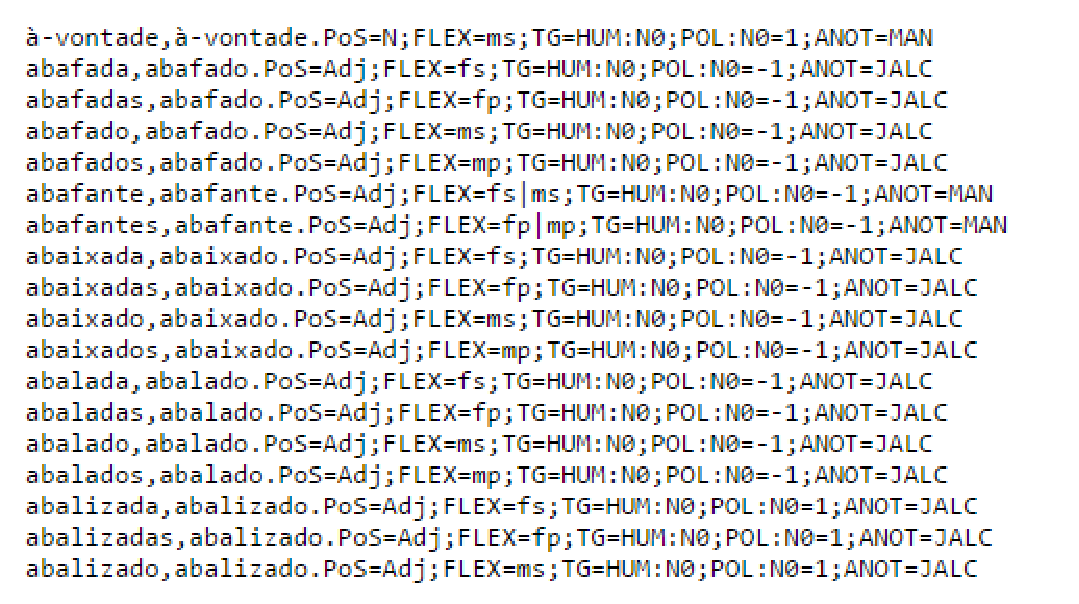
\epsfig{file=figuras/sentilex.eps, width=15cm}
	\caption{Base SentiLex-PT antes da normalização}
	\label{sentilex}
\end{figure}

E após a divisão dos termos positivos e negativos em arquivos distintos, o resultado segue abaixo:


\begin{figure}[H]
	
	\center
	\subfigure[sentilexpos][Lista de termos positivos]{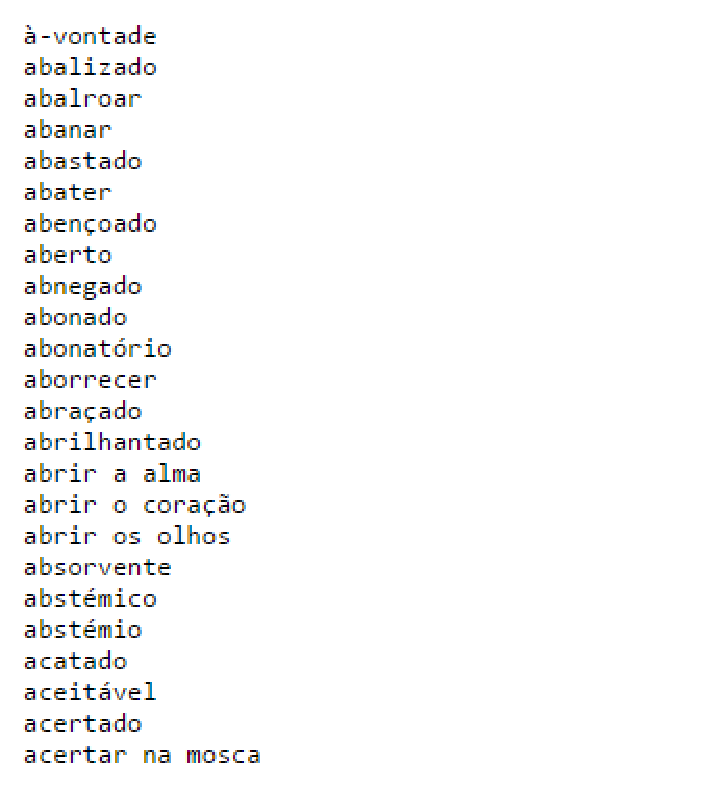
\includegraphics[width=7cm]{figuras/sentilexpos.eps}}
	\qquad
	\subfigure[sentilexneg][Lista de termos negativos]{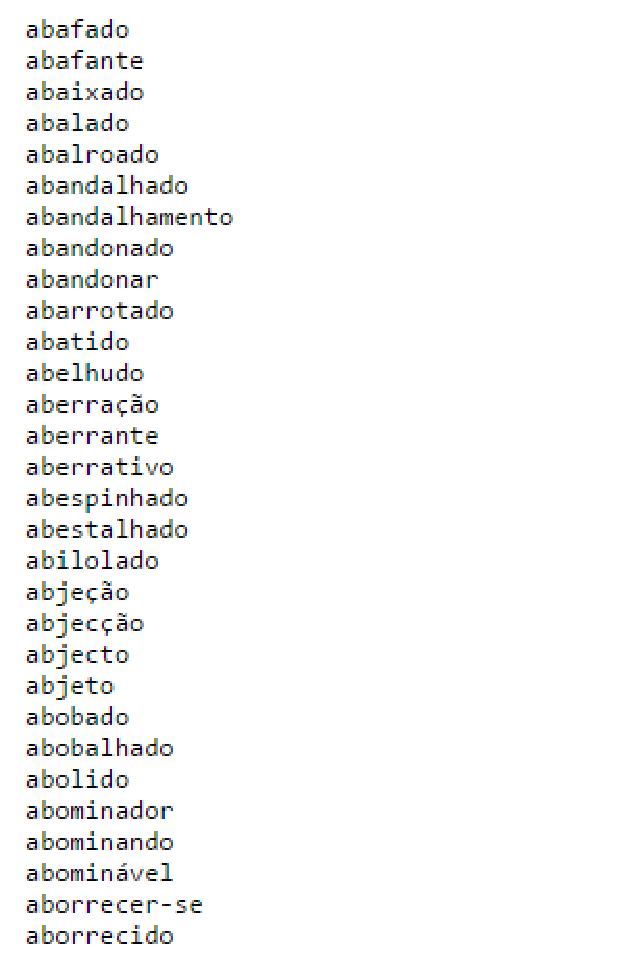
\includegraphics[width=7cm]{figuras/sentilexneg.eps}}
	\caption{Base SentiLex-PT normalizada, dividindo em dois arquivos distintos os termos positivos e negativos}
	
\end{figure}

Por último, durante os testes com a classificação surgiu a ideia de produzir uma base de dados customizada para o evento Oscar 2016. A base de dados foi elaborada seguindo o padrão estabelecido anteriormente e preenchida com palavras relevantes ao contexto do evento e classificadas manualmente pelo idealizadores deste projeto.

\begin{figure}[H]
	
	\center
	\subfigure[oscar-pos][Lista de termos positivas]{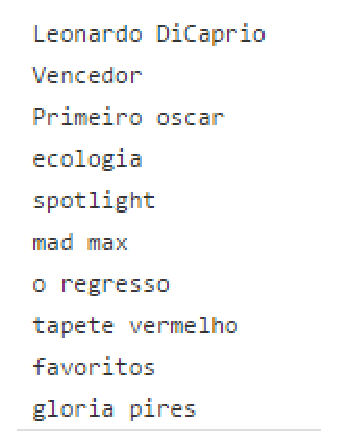
\includegraphics[width=5cm]{figuras/oscar-pos.eps}}
	\qquad
	\subfigure[oscar-neg][Lista de termos negativas]{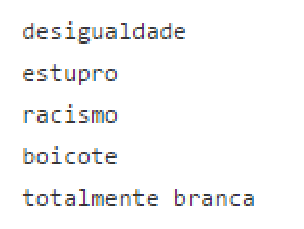
\includegraphics[width=5cm]{figuras/oscar-neg.eps}}
	\caption{Amostragem da base de termos \textit{Oscar 2016} normalizada, dividindo em dois arquivos distintos os termos positivos e negativos}
	
\end{figure}

\subsection{Aplicação do algoritmo Naive Bayes}
O primeiro passo para a classificação de um \textit{tweet} é calibrar o algoritmo escolhido para efetuar a classificação - lembrando que para este trabalho foi utilizado o algoritmo \textit{Naive Bayes}. Com posse das bases de palavras e termos já classificados anteriormente foi necessário treinar o algoritmo para que ele conseguisse se calibrar através das palavras e termos classificados contidos nas bases. 
Como já foi abordado anteriormente, para este projeto foi utilizada a biblioteca NLTK, construída como suíte de soluções para trabalhar com linguagem natural para Python. O NLTK possui diversos algoritmos de classificação disponíveis para uso, sendo o \textit{Naive Bayes} um deles.

Por padrão, para treinar o algoritmo, o NLTK utiliza como base de dados alguns bancos de palavras genéricas disponíveis dentro da própria biblioteca. Para utilizar as bases de dados mencionadas acima como massa de treino para o algoritmo foi necessário sobrescrever os métodos de treino do classificador contidos dentro do NLTK. Após esta customização, o algoritmo passou a classificar textos utilizando as bases descritas acima como massa de treino.

Como resultado da classificação, o \textit{Naive Bayes} retorna dois valores como resultado: o primeiro sendo a probabilidade entre zero e um do texto classificado ser positivo e outro sendo a probabilidade do mesmo ser negativo. A soma entre as duas probabilidades sempre resultam em um. Exemplo:

\begin{lstlisting}[style=python, frame=single]
In[1]: from classifier import SentmentClassifier
In[2]: sentiment = SentimentClassifier.classify("Spotlight foi sensacional! #oscars2016")
In[3]: print sentiment

Out[1]: Sentiment({p_pos: 0.91, p_neg: 0.09, classification: "pos"})

\end{lstlisting}

Durante testes com o algoritmo de classificação \textit{Naive Bayes} foi observado que quando o mesmo não conseguia extrair nenhuma tendência positiva ou negativa do texto a ser classificado o resultado determinava uma probabilidade igual do texto ser positivo ou negativo. Por este motivo, para facilitar as consultas e análises posteriores foi feita uma ligeira modificação para salvar o sentimento nesses casos como \textit{"neu"} - uma alusão a palavra \textit{"neutro"}.

Como foi dito anteriormente na seção \ref{proposta:armazenamento} antes de armazenar o documento extraído da API do Twitter são adicionadas algumas informações pertinentes ao processo de classificação. Entre elas podemos citar:

\begin{itemize}
	\item \textit{\textbf{normalized\_text}} texto normalizado sem \textit{stopwords} e apenas contendo o radical de cada palavra do \textit{tweet};
	\item \textit{\textbf{classification}}: classificação semântica que pode variar em positiva, neutra ou negativa;
	\item \textit{\textbf{p\_pos}}: probabilidade do texto classificado ser positivo segundo o algoritmo;
	\item \textit{\textbf{p\_neg}}: probabilidade do texto classificado ser negativo segundo o algoritmo;
	\item \textit{\textbf{databases}}: bancos de dados de palavras utilizados como masse de treino para a classificação;
	\item \textit{\textbf{classified\_at}}: data e hora da classificação.
\end{itemize}

Estas informações foram incluídas por serem consideradas úteis durante o processo de análise dos resultados - tornando a consulta na base de dados mais simples - e durante o processo de análise do desempenho do algoritmo escolhido - mostrando por exemplo quais bases de palavras se mostraram mais eficientes para o estudo de caso conduzido durante o evento de entrega do Oscar 2016, entre outras métricas e análises que serão abordadas no Capítulo 4. 

Por se tratar de algoritmo baixa complexidade matemática, o processo de classificação se mostrou surpreendentemente rápido e não se mostrou um gargalo para o processo de coleta de dados no Twitter, que apenas precisa buscar os últimos \textit{tweets} na API do Twitter. Por conta disso, foi possível extrair os \textit{tweets} e classificá-los imediatamente sem atrasar ou prejudicar a etapa de coleta.